\documentclass[1p]{elsarticle_modified}
%\bibliographystyle{elsarticle-num}

%\usepackage[colorlinks]{hyperref}
%\usepackage{abbrmath_seonhwa} %\Abb, \Ascr, \Acal ,\Abf, \Afrak
\usepackage{amsfonts}
\usepackage{amssymb}
\usepackage{amsmath}
\usepackage{amsthm}
\usepackage{scalefnt}
\usepackage{amsbsy}
\usepackage{kotex}
\usepackage{caption}
\usepackage{subfig}
\usepackage{color}
\usepackage{graphicx}
\usepackage{xcolor} %% white, black, red, green, blue, cyan, magenta, yellow
\usepackage{float}
\usepackage{setspace}
\usepackage{hyperref}

\usepackage{tikz}
\usetikzlibrary{arrows}

\usepackage{multirow}
\usepackage{array} % fixed length table
\usepackage{hhline}

%%%%%%%%%%%%%%%%%%%%%
\makeatletter
\renewcommand*\env@matrix[1][\arraystretch]{%
	\edef\arraystretch{#1}%
	\hskip -\arraycolsep
	\let\@ifnextchar\new@ifnextchar
	\array{*\c@MaxMatrixCols c}}
\makeatother %https://tex.stackexchange.com/questions/14071/how-can-i-increase-the-line-spacing-in-a-matrix
%%%%%%%%%%%%%%%

\usepackage[normalem]{ulem}

\newcommand{\msout}[1]{\ifmmode\text{\sout{\ensuremath{#1}}}\else\sout{#1}\fi}
%SOURCE: \msout is \stkout macro in https://tex.stackexchange.com/questions/20609/strikeout-in-math-mode

\newcommand{\cancel}[1]{
	\ifmmode
	{\color{red}\msout{#1}}
	\else
	{\color{red}\sout{#1}}
	\fi
}

\newcommand{\add}[1]{
	{\color{blue}\uwave{#1}}
}

\newcommand{\replace}[2]{
	\ifmmode
	{\color{red}\msout{#1}}{\color{blue}\uwave{#2}}
	\else
	{\color{red}\sout{#1}}{\color{blue}\uwave{#2}}
	\fi
}

\newcommand{\Sol}{\mathcal{S}} %segment
\newcommand{\D}{D} %diagram
\newcommand{\A}{\mathcal{A}} %arc


%%%%%%%%%%%%%%%%%%%%%%%%%%%%%5 test

\def\sl{\operatorname{\textup{SL}}(2,\Cbb)}
\def\psl{\operatorname{\textup{PSL}}(2,\Cbb)}
\def\quan{\mkern 1mu \triangleright \mkern 1mu}

\theoremstyle{definition}
\newtheorem{thm}{Theorem}[section]
\newtheorem{prop}[thm]{Proposition}
\newtheorem{lem}[thm]{Lemma}
\newtheorem{ques}[thm]{Question}
\newtheorem{cor}[thm]{Corollary}
\newtheorem{defn}[thm]{Definition}
\newtheorem{exam}[thm]{Example}
\newtheorem{rmk}[thm]{Remark}
\newtheorem{alg}[thm]{Algorithm}

\newcommand{\I}{\sqrt{-1}}
\begin{document}

%\begin{frontmatter}
%
%\title{Boundary parabolic representations of knots up to 8 crossings}
%
%%% Group authors per affiliation:
%\author{Yunhi Cho} 
%\address{Department of Mathematics, University of Seoul, Seoul, Korea}
%\ead{yhcho@uos.ac.kr}
%
%
%\author{Seonhwa Kim} %\fnref{s_kim}}
%\address{Center for Geometry and Physics, Institute for Basic Science, Pohang, 37673, Korea}
%\ead{ryeona17@ibs.re.kr}
%
%\author{Hyuk Kim}
%\address{Department of Mathematical Sciences, Seoul National University, Seoul 08826, Korea}
%\ead{hyukkim@snu.ac.kr}
%
%\author{Seokbeom Yoon}
%\address{Department of Mathematical Sciences, Seoul National University, Seoul, 08826,  Korea}
%\ead{sbyoon15@snu.ac.kr}
%
%\begin{abstract}
%We find all boundary parabolic representation of knots up to 8 crossings.
%
%\end{abstract}
%\begin{keyword}
%    \MSC[2010] 57M25 
%\end{keyword}
%
%\end{frontmatter}

%\linenumbers
%\tableofcontents
%
\newcommand\colored[1]{\textcolor{white}{\rule[-0.35ex]{0.8em}{1.4ex}}\kern-0.8em\color{red} #1}%
%\newcommand\colored[1]{\textcolor{white}{ #1}\kern-2.17ex	\textcolor{white}{ #1}\kern-1.81ex	\textcolor{white}{ #1}\kern-2.15ex\color{red}#1	}

{\Large $\underline{11a_{173}~(K11a_{173})}$}

\setlength{\tabcolsep}{10pt}
\renewcommand{\arraystretch}{1.6}
\vspace{1cm}\begin{tabular}{m{100pt}>{\centering\arraybackslash}m{274pt}}
\multirow{5}{120pt}{
	\centering
	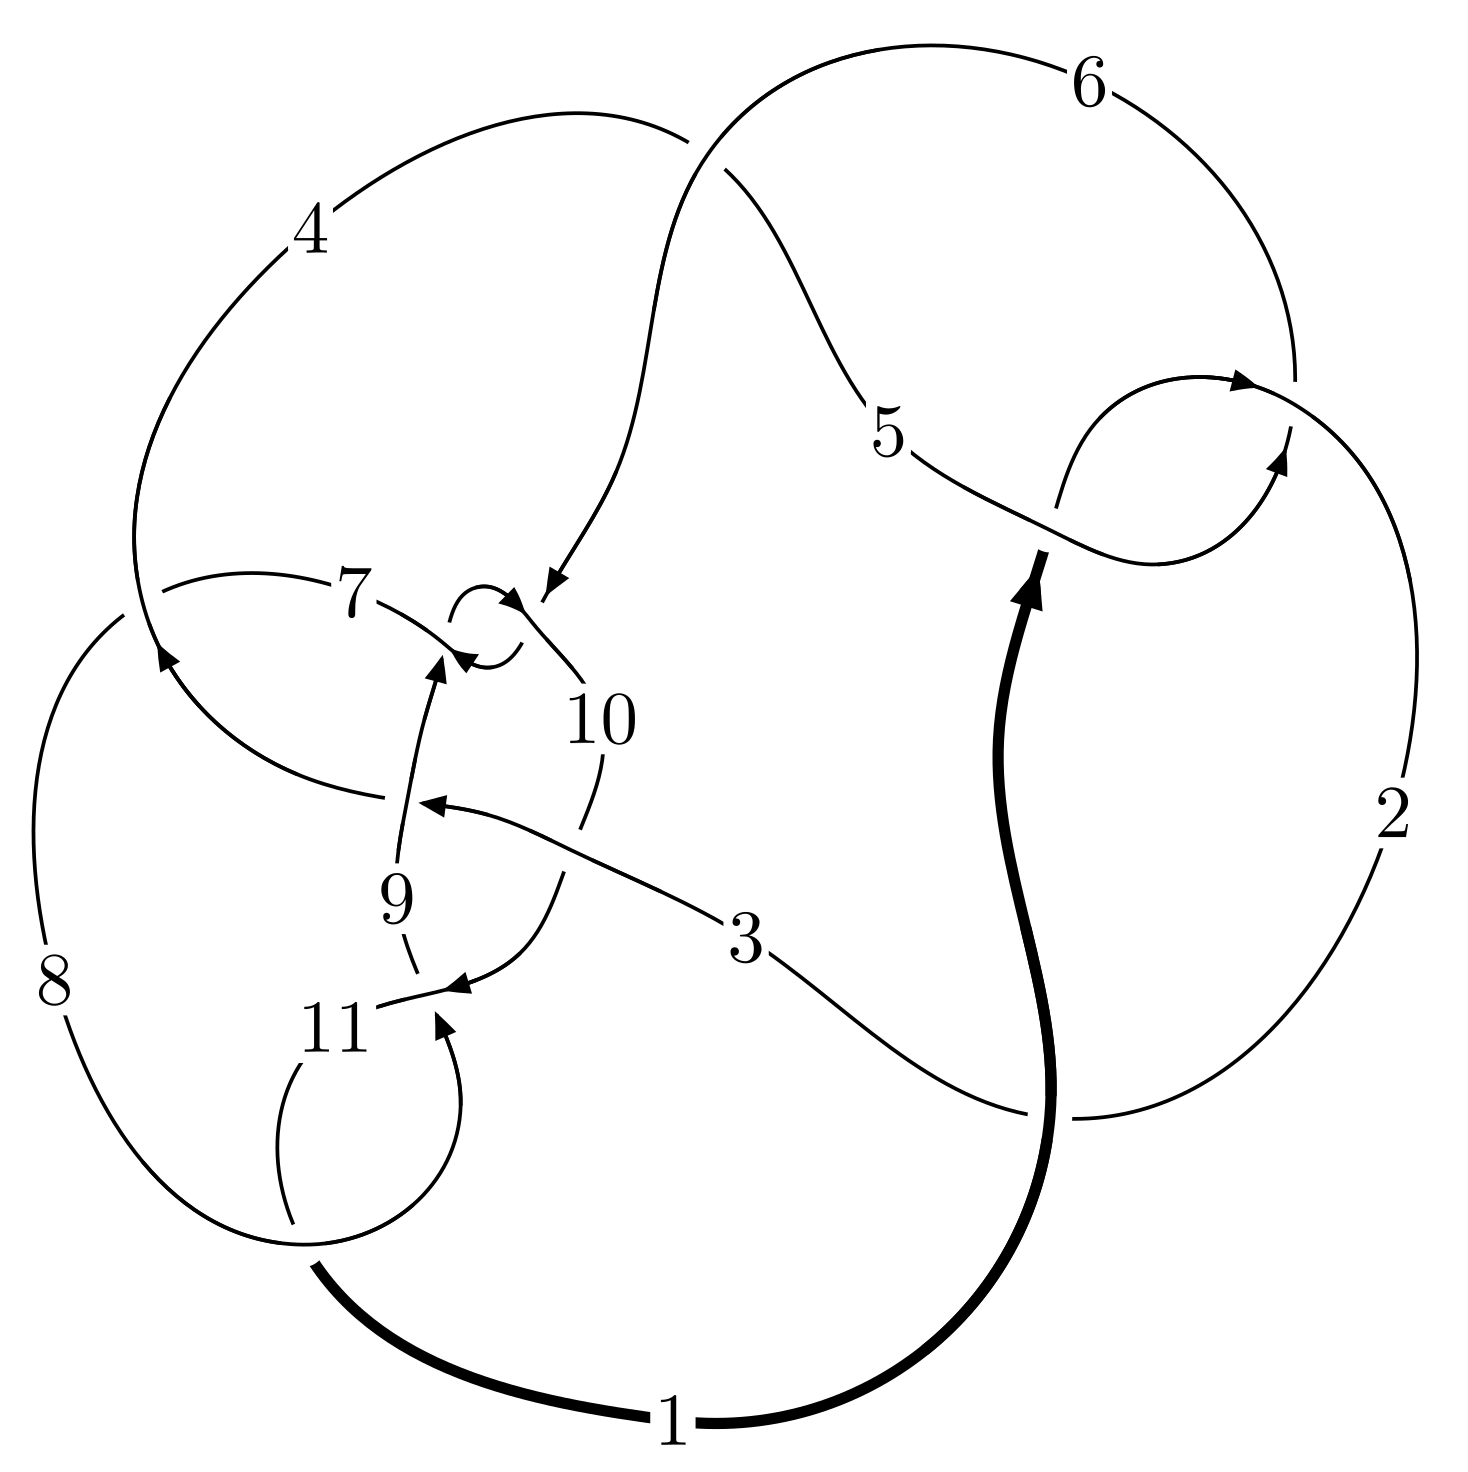
\includegraphics[width=112pt]{../../../GIT/diagram.site/Diagrams/png/422_11a_173.png}\\
\ \ \ A knot diagram\footnotemark}&
\allowdisplaybreaks
\textbf{Linearized knot diagam} \\
\cline{2-2}
 &
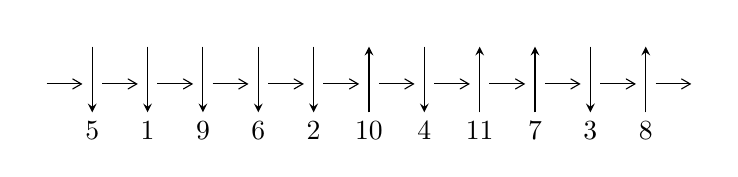
\begin{tikzpicture}[x=20pt, y=17pt]
	% nodes
	\node (C0) at (0, 0) {};
	\node (C1) at (1, 0) {};
	\node (C1U) at (1, +1) {};
	\node (C1D) at (1, -1) {5};

	\node (C2) at (2, 0) {};
	\node (C2U) at (2, +1) {};
	\node (C2D) at (2, -1) {1};

	\node (C3) at (3, 0) {};
	\node (C3U) at (3, +1) {};
	\node (C3D) at (3, -1) {9};

	\node (C4) at (4, 0) {};
	\node (C4U) at (4, +1) {};
	\node (C4D) at (4, -1) {6};

	\node (C5) at (5, 0) {};
	\node (C5U) at (5, +1) {};
	\node (C5D) at (5, -1) {2};

	\node (C6) at (6, 0) {};
	\node (C6U) at (6, +1) {};
	\node (C6D) at (6, -1) {10};

	\node (C7) at (7, 0) {};
	\node (C7U) at (7, +1) {};
	\node (C7D) at (7, -1) {4};

	\node (C8) at (8, 0) {};
	\node (C8U) at (8, +1) {};
	\node (C8D) at (8, -1) {11};

	\node (C9) at (9, 0) {};
	\node (C9U) at (9, +1) {};
	\node (C9D) at (9, -1) {7};

	\node (C10) at (10, 0) {};
	\node (C10U) at (10, +1) {};
	\node (C10D) at (10, -1) {3};

	\node (C11) at (11, 0) {};
	\node (C11U) at (11, +1) {};
	\node (C11D) at (11, -1) {8};
	\node (C12) at (12, 0) {};

	% arrows
	\draw[->,>={angle 60}]
	(C0) edge (C1) (C1) edge (C2) (C2) edge (C3) (C3) edge (C4) (C4) edge (C5) (C5) edge (C6) (C6) edge (C7) (C7) edge (C8) (C8) edge (C9) (C9) edge (C10) (C10) edge (C11) (C11) edge (C12) ;	\draw[->,>=stealth]
	(C1U) edge (C1D) (C2U) edge (C2D) (C3U) edge (C3D) (C4U) edge (C4D) (C5U) edge (C5D) (C6D) edge (C6U) (C7U) edge (C7D) (C8D) edge (C8U) (C9D) edge (C9U) (C10U) edge (C10D) (C11D) edge (C11U) ;
	\end{tikzpicture} \\
\hhline{~~} \\& 
\textbf{Solving Sequence} \\ \cline{2-2} 
 &
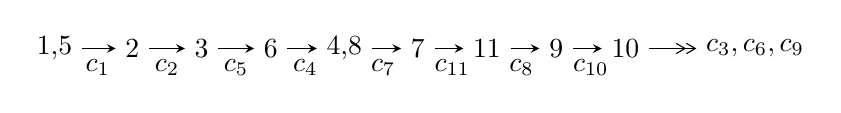
\begin{tikzpicture}[x=25pt, y=7pt]
	% node
	\node (A0) at (-1/8, 0) {1,5};
	\node (A1) at (1, 0) {2};
	\node (A2) at (2, 0) {3};
	\node (A3) at (3, 0) {6};
	\node (A4) at (65/16, 0) {4,8};
	\node (A5) at (41/8, 0) {7};
	\node (A6) at (49/8, 0) {11};
	\node (A7) at (57/8, 0) {9};
	\node (A8) at (65/8, 0) {10};
	\node (C1) at (1/2, -1) {$c_{1}$};
	\node (C2) at (3/2, -1) {$c_{2}$};
	\node (C3) at (5/2, -1) {$c_{5}$};
	\node (C4) at (7/2, -1) {$c_{4}$};
	\node (C5) at (37/8, -1) {$c_{7}$};
	\node (C6) at (45/8, -1) {$c_{11}$};
	\node (C7) at (53/8, -1) {$c_{8}$};
	\node (C8) at (61/8, -1) {$c_{10}$};
	\node (A9) at (10, 0) {$c_{3},c_{6},c_{9}$};

	% edge
	\draw[->,>=stealth]	
	(A0) edge (A1) (A1) edge (A2) (A2) edge (A3) (A3) edge (A4) (A4) edge (A5) (A5) edge (A6) (A6) edge (A7) (A7) edge (A8) ;
	\draw[->>,>={angle 60}]	
	(A8) edge (A9);
\end{tikzpicture} \\ 

\end{tabular} \\

\footnotetext{
The image of knot diagram is generated by the software ``\textbf{Draw programme}" developed by Andrew Bartholomew(\url{http://www.layer8.co.uk/maths/draw/index.htm\#Running-draw}), where we modified some parts for our purpose(\url{https://github.com/CATsTAILs/LinksPainter}).
}\phantom \\ \newline 
\centering \textbf{Ideals for irreducible components\footnotemark of $X_{\text{par}}$} 
 
\begin{align*}
I^u_{1}&=\langle 
-14767307395 u^{27}+20235323073 u^{26}+\cdots+98330713818 b+33355375098,\\
\phantom{I^u_{1}}&\phantom{= \langle  }32428293291 u^{27}-21218621420 u^{26}+\cdots+196661427636 a+204360671755,\\
\phantom{I^u_{1}}&\phantom{= \langle  }u^{28}-2 u^{27}+\cdots-3 u-4\rangle \\
I^u_{2}&=\langle 
- u^4 a- u^3 a+14 u^4-2 u^2 a-5 u^3-4 a u-10 u^2+19 b+9 a- u+26,\\
\phantom{I^u_{2}}&\phantom{= \langle  }5 u^4 a-2 u^3 a+16 u^4- u^2 a-8 u^3+a^2- a u-5 u^2+9 a-3 u+30,\;u^5- u^4+2 u-1\rangle \\
I^u_{3}&=\langle 
19 u^{15} a+23 u^{15}+\cdots+20 a+27,\;2 u^{15} a+6 u^{15}+\cdots+a^2-4,\\
\phantom{I^u_{3}}&\phantom{= \langle  }u^{16}- u^{15}-2 u^{14}+3 u^{13}+4 u^{12}-7 u^{11}-3 u^{10}+10 u^9-9 u^7+3 u^6+5 u^5-4 u^4+2 u^2-2 u+1\rangle \\
I^u_{4}&=\langle 
b-1,\;2 a-2 u+1,\;u^3+u^2-1\rangle \\
I^u_{5}&=\langle 
b- a-1,\;a^2+a+2,\;u+1\rangle \\
I^u_{6}&=\langle 
2 b- a+1,\;a^2-2 a+5,\;u-1\rangle \\
\\
\end{align*}
\raggedright * 6 irreducible components of $\dim_{\mathbb{C}}=0$, with total 77 representations.\\
\footnotetext{All coefficients of polynomials are rational numbers. But the coefficients are sometimes approximated in decimal forms when there is not enough margin.}
\newpage
\renewcommand{\arraystretch}{1}
\centering \section*{I. $I^u_{1}= \langle -1.48\times10^{10} u^{27}+2.02\times10^{10} u^{26}+\cdots+9.83\times10^{10} b+3.34\times10^{10},\;3.24\times10^{10} u^{27}-2.12\times10^{10} u^{26}+\cdots+1.97\times10^{11} a+2.04\times10^{11},\;u^{28}-2 u^{27}+\cdots-3 u-4 \rangle$}
\flushleft \textbf{(i) Arc colorings}\\
\begin{tabular}{m{7pt} m{180pt} m{7pt} m{180pt} }
\flushright $a_{1}=$&$\begin{pmatrix}1\\0\end{pmatrix}$ \\
\flushright $a_{5}=$&$\begin{pmatrix}0\\u\end{pmatrix}$ \\
\flushright $a_{2}=$&$\begin{pmatrix}1\\u^2\end{pmatrix}$ \\
\flushright $a_{3}=$&$\begin{pmatrix}- u^2+1\\u^2\end{pmatrix}$ \\
\flushright $a_{6}=$&$\begin{pmatrix}- u\\- u^3+u\end{pmatrix}$ \\
\flushright $a_{4}=$&$\begin{pmatrix}u^3\\u^5- u^3+u\end{pmatrix}$ \\
\flushright $a_{8}=$&$\begin{pmatrix}-0.164894 u^{27}+0.107894 u^{26}+\cdots-2.21519 u-1.03915\\0.150180 u^{27}-0.205788 u^{26}+\cdots+0.595130 u-0.339216\end{pmatrix}$ \\
\flushright $a_{7}=$&$\begin{pmatrix}-0.160609 u^{27}+0.110297 u^{26}+\cdots-2.13491 u-1.03465\\0.227707 u^{27}-0.221295 u^{26}+\cdots+0.789310 u-0.0177292\end{pmatrix}$ \\
\flushright $a_{11}=$&$\begin{pmatrix}0.206489 u^{27}-0.182794 u^{26}+\cdots+1.38239 u+1.44504\\-0.198851 u^{27}+0.240301 u^{26}+\cdots+0.0000310478 u+0.278301\end{pmatrix}$ \\
\flushright $a_{9}=$&$\begin{pmatrix}-0.312509 u^{27}+0.216909 u^{26}+\cdots-2.81796 u-1.93782\\0.373802 u^{27}-0.449982 u^{26}+\cdots+0.400981 u-0.382402\end{pmatrix}$ \\
\flushright $a_{10}=$&$\begin{pmatrix}0.137090 u^{27}-0.0589378 u^{26}+\cdots+1.47329 u+1.50912\\-0.199975 u^{27}+0.238265 u^{26}+\cdots-0.339747 u+0.201391\end{pmatrix}$\\ \flushright $a_{10}=$&$\begin{pmatrix}0.137090 u^{27}-0.0589378 u^{26}+\cdots+1.47329 u+1.50912\\-0.199975 u^{27}+0.238265 u^{26}+\cdots-0.339747 u+0.201391\end{pmatrix}$\\&\end{tabular}
\flushleft \textbf{(ii) Obstruction class $= -1$}\\~\\
\flushleft \textbf{(iii) Cusp Shapes $= -\frac{138939169865}{196661427636} u^{27}-\frac{31573928977}{196661427636} u^{26}+\cdots-\frac{326662110881}{16388452303} u-\frac{420010681258}{49165356909}$}\\~\\
\newpage\renewcommand{\arraystretch}{1}
\flushleft \textbf{(iv) u-Polynomials at the component}\newline \\
\begin{tabular}{m{50pt}|m{274pt}}
Crossings & \hspace{64pt}u-Polynomials at each crossing \\
\hline $$\begin{aligned}c_{1},c_{5}\end{aligned}$$&$\begin{aligned}
&u^{28}+2 u^{27}+\cdots+3 u-4
\end{aligned}$\\
\hline $$\begin{aligned}c_{2},c_{4}\end{aligned}$$&$\begin{aligned}
&u^{28}+10 u^{27}+\cdots+97 u+16
\end{aligned}$\\
\hline $$\begin{aligned}c_{3}\end{aligned}$$&$\begin{aligned}
&u^{28}+3 u^{27}+\cdots+736 u+128
\end{aligned}$\\
\hline $$\begin{aligned}c_{6},c_{8},c_{9}\\c_{11}\end{aligned}$$&$\begin{aligned}
&u^{28}-3 u^{27}+\cdots-5 u-1
\end{aligned}$\\
\hline $$\begin{aligned}c_{7},c_{10}\end{aligned}$$&$\begin{aligned}
&8(8 u^{28}-12 u^{27}+\cdots+4 u+2)
\end{aligned}$\\
\hline
\end{tabular}\\~\\
\newpage\renewcommand{\arraystretch}{1}
\flushleft \textbf{(v) Riley Polynomials at the component}\newline \\
\begin{tabular}{m{50pt}|m{274pt}}
Crossings & \hspace{64pt}Riley Polynomials at each crossing \\
\hline $$\begin{aligned}c_{1},c_{5}\end{aligned}$$&$\begin{aligned}
&y^{28}-10 y^{27}+\cdots-97 y+16
\end{aligned}$\\
\hline $$\begin{aligned}c_{2},c_{4}\end{aligned}$$&$\begin{aligned}
&y^{28}+18 y^{27}+\cdots+8543 y+256
\end{aligned}$\\
\hline $$\begin{aligned}c_{3}\end{aligned}$$&$\begin{aligned}
&y^{28}-5 y^{27}+\cdots-238592 y+16384
\end{aligned}$\\
\hline $$\begin{aligned}c_{6},c_{8},c_{9}\\c_{11}\end{aligned}$$&$\begin{aligned}
&y^{28}+11 y^{27}+\cdots-51 y+1
\end{aligned}$\\
\hline $$\begin{aligned}c_{7},c_{10}\end{aligned}$$&$\begin{aligned}
&64(64 y^{28}+176 y^{27}+\cdots+40 y+4)
\end{aligned}$\\
\hline
\end{tabular}\\~\\
\newpage\flushleft \textbf{(vi) Complex Volumes and Cusp Shapes}
$$\begin{array}{c|c|c}  
\text{Solutions to }I^u_{1}& \I (\text{vol} + \sqrt{-1}CS) & \text{Cusp shape}\\
 \hline 
\begin{aligned}
u &= -0.566116 + 0.813544 I \\
a &= \phantom{-}0.534639 - 0.137883 I \\
b &= -0.471357 + 0.915613 I\end{aligned}
 & \phantom{-}1.74883 - 2.81556 I & -1.14300 + 4.42775 I \\ \hline\begin{aligned}
u &= -0.566116 - 0.813544 I \\
a &= \phantom{-}0.534639 + 0.137883 I \\
b &= -0.471357 - 0.915613 I\end{aligned}
 & \phantom{-}1.74883 + 2.81556 I & -1.14300 - 4.42775 I \\ \hline\begin{aligned}
u &= \phantom{-}0.805429 + 0.748611 I \\
a &= \phantom{-}1.99187 + 0.34421 I \\
b &= -1.193820 + 0.462931 I\end{aligned}
 & \phantom{-}4.99503 - 1.79073 I & -1.05075 - 2.61493 I \\ \hline\begin{aligned}
u &= \phantom{-}0.805429 - 0.748611 I \\
a &= \phantom{-}1.99187 - 0.34421 I \\
b &= -1.193820 - 0.462931 I\end{aligned}
 & \phantom{-}4.99503 + 1.79073 I & -1.05075 + 2.61493 I \\ \hline\begin{aligned}
u &= \phantom{-}0.679059 + 0.893968 I \\
a &= -0.932511 - 0.786849 I \\
b &= \phantom{-}0.600465 + 1.265070 I\end{aligned}
 & -0.89815 + 10.64770 I & -3.82752 - 5.52190 I \\ \hline\begin{aligned}
u &= \phantom{-}0.679059 - 0.893968 I \\
a &= -0.932511 + 0.786849 I \\
b &= \phantom{-}0.600465 - 1.265070 I\end{aligned}
 & -0.89815 - 10.64770 I & -3.82752 + 5.52190 I \\ \hline\begin{aligned}
u &= \phantom{-}0.167815 + 0.852338 I \\
a &= -0.800362 + 0.593310 I \\
b &= \phantom{-}0.442426 - 1.154500 I\end{aligned}
 & -3.88792 - 6.82425 I & -4.62158 + 6.71855 I \\ \hline\begin{aligned}
u &= \phantom{-}0.167815 - 0.852338 I \\
a &= -0.800362 - 0.593310 I \\
b &= \phantom{-}0.442426 + 1.154500 I\end{aligned}
 & -3.88792 + 6.82425 I & -4.62158 - 6.71855 I \\ \hline\begin{aligned}
u &= -0.838400\phantom{ +0.000000I} \\
a &= -0.287249\phantom{ +0.000000I} \\
b &= -1.20069\phantom{ +0.000000I}\end{aligned}
 & \phantom{-}0.271501\phantom{ +0.000000I} & -23.7360\phantom{ +0.000000I} \\ \hline\begin{aligned}
u &= -1.156720 + 0.209637 I \\
a &= -0.79174 + 1.21845 I \\
b &= \phantom{-}0.465804 + 1.280600 I\end{aligned}
 & -8.43358 + 10.19260 I & -10.18832 - 7.63922 I\\
 \hline 
 \end{array}$$\newpage$$\begin{array}{c|c|c}  
\text{Solutions to }I^u_{1}& \I (\text{vol} + \sqrt{-1}CS) & \text{Cusp shape}\\
 \hline 
\begin{aligned}
u &= -1.156720 - 0.209637 I \\
a &= -0.79174 - 1.21845 I \\
b &= \phantom{-}0.465804 - 1.280600 I\end{aligned}
 & -8.43358 - 10.19260 I & -10.18832 + 7.63922 I \\ \hline\begin{aligned}
u &= \phantom{-}0.928400 + 0.721425 I \\
a &= \phantom{-}1.19972 + 1.35918 I \\
b &= -1.278550 - 0.388894 I\end{aligned}
 & \phantom{-}4.61539 - 3.79849 I & -3.70384 + 8.50950 I \\ \hline\begin{aligned}
u &= \phantom{-}0.928400 - 0.721425 I \\
a &= \phantom{-}1.19972 - 1.35918 I \\
b &= -1.278550 + 0.388894 I\end{aligned}
 & \phantom{-}4.61539 + 3.79849 I & -3.70384 - 8.50950 I \\ \hline\begin{aligned}
u &= -0.878060 + 0.825409 I \\
a &= -0.366900 + 0.450231 I \\
b &= \phantom{-}0.338313 - 0.571686 I\end{aligned}
 & \phantom{-}3.34352 + 1.62496 I & -2.45048 + 1.41829 I \\ \hline\begin{aligned}
u &= -0.878060 - 0.825409 I \\
a &= -0.366900 - 0.450231 I \\
b &= \phantom{-}0.338313 + 0.571686 I\end{aligned}
 & \phantom{-}3.34352 - 1.62496 I & -2.45048 - 1.41829 I \\ \hline\begin{aligned}
u &= \phantom{-}1.214650 + 0.097151 I \\
a &= -0.222900 - 0.987308 I \\
b &= -0.155309 - 0.849372 I\end{aligned}
 & -4.05629 + 0.93128 I & -2.23485 - 6.88947 I \\ \hline\begin{aligned}
u &= \phantom{-}1.214650 - 0.097151 I \\
a &= -0.222900 + 0.987308 I \\
b &= -0.155309 + 0.849372 I\end{aligned}
 & -4.05629 - 0.93128 I & -2.23485 + 6.88947 I \\ \hline\begin{aligned}
u &= -0.903785 + 0.845201 I \\
a &= -1.078650 - 0.117582 I \\
b &= \phantom{-}0.379054 + 0.705257 I\end{aligned}
 & \phantom{-}3.28350 + 4.57627 I & -2.13594 - 7.47854 I \\ \hline\begin{aligned}
u &= -0.903785 - 0.845201 I \\
a &= -1.078650 + 0.117582 I \\
b &= \phantom{-}0.379054 - 0.705257 I\end{aligned}
 & \phantom{-}3.28350 - 4.57627 I & -2.13594 + 7.47854 I \\ \hline\begin{aligned}
u &= \phantom{-}1.168360 + 0.434244 I \\
a &= \phantom{-}0.627774 + 0.344147 I \\
b &= \phantom{-}0.309881 + 1.145950 I\end{aligned}
 & -7.10420 + 2.17526 I & -9.93897 - 4.23335 I\\
 \hline 
 \end{array}$$\newpage$$\begin{array}{c|c|c}  
\text{Solutions to }I^u_{1}& \I (\text{vol} + \sqrt{-1}CS) & \text{Cusp shape}\\
 \hline 
\begin{aligned}
u &= \phantom{-}1.168360 - 0.434244 I \\
a &= \phantom{-}0.627774 - 0.344147 I \\
b &= \phantom{-}0.309881 - 1.145950 I\end{aligned}
 & -7.10420 - 2.17526 I & -9.93897 + 4.23335 I \\ \hline\begin{aligned}
u &= -1.074080 + 0.691225 I \\
a &= \phantom{-}1.41798 - 0.69280 I \\
b &= -0.422318 - 1.038380 I\end{aligned}
 & \phantom{-}0.23866 + 8.48658 I & -4.72348 - 9.14479 I \\ \hline\begin{aligned}
u &= -1.074080 - 0.691225 I \\
a &= \phantom{-}1.41798 + 0.69280 I \\
b &= -0.422318 + 1.038380 I\end{aligned}
 & \phantom{-}0.23866 - 8.48658 I & -4.72348 + 9.14479 I \\ \hline\begin{aligned}
u &= \phantom{-}1.050060 + 0.753206 I \\
a &= -2.17570 - 0.35594 I \\
b &= \phantom{-}0.60850 - 1.30717 I\end{aligned}
 & -2.0462 - 16.7456 I & -5.37386 + 9.80445 I \\ \hline\begin{aligned}
u &= \phantom{-}1.050060 - 0.753206 I \\
a &= -2.17570 + 0.35594 I \\
b &= \phantom{-}0.60850 + 1.30717 I\end{aligned}
 & -2.0462 + 16.7456 I & -5.37386 - 9.80445 I \\ \hline\begin{aligned}
u &= \phantom{-}0.682847\phantom{ +0.000000I} \\
a &= -0.725706\phantom{ +0.000000I} \\
b &= \phantom{-}0.129567\phantom{ +0.000000I}\end{aligned}
 & -0.926639\phantom{ +0.000000I} & -11.5880\phantom{ +0.000000I} \\ \hline\begin{aligned}
u &= -0.357231 + 0.322552 I \\
a &= \phantom{-}0.478268 - 0.914294 I \\
b &= -0.587531 - 0.365743 I\end{aligned}
 & \phantom{-}1.12674 + 1.01957 I & \phantom{-}4.42993 - 4.67672 I \\ \hline\begin{aligned}
u &= -0.357231 - 0.322552 I \\
a &= \phantom{-}0.478268 + 0.914294 I \\
b &= -0.587531 + 0.365743 I\end{aligned}
 & \phantom{-}1.12674 - 1.01957 I & \phantom{-}4.42993 + 4.67672 I\\
 \hline 
 \end{array}$$\newpage\newpage\renewcommand{\arraystretch}{1}
\centering \section*{II. $I^u_{2}= \langle - u^4 a+14 u^4+\cdots+9 a+26,\;5 u^4 a+16 u^4+\cdots+9 a+30,\;u^5- u^4+2 u-1 \rangle$}
\flushleft \textbf{(i) Arc colorings}\\
\begin{tabular}{m{7pt} m{180pt} m{7pt} m{180pt} }
\flushright $a_{1}=$&$\begin{pmatrix}1\\0\end{pmatrix}$ \\
\flushright $a_{5}=$&$\begin{pmatrix}0\\u\end{pmatrix}$ \\
\flushright $a_{2}=$&$\begin{pmatrix}1\\u^2\end{pmatrix}$ \\
\flushright $a_{3}=$&$\begin{pmatrix}- u^2+1\\u^2\end{pmatrix}$ \\
\flushright $a_{6}=$&$\begin{pmatrix}- u\\- u^3+u\end{pmatrix}$ \\
\flushright $a_{4}=$&$\begin{pmatrix}u^3\\u^4- u^3- u+1\end{pmatrix}$ \\
\flushright $a_{8}=$&$\begin{pmatrix}a\\0.0526316 a u^{4}-0.736842 u^{4}+\cdots-0.473684 a-1.36842\end{pmatrix}$ \\
\flushright $a_{7}=$&$\begin{pmatrix}0.368421 a u^{4}-0.157895 u^{4}+\cdots+0.684211 a+0.421053\\- u^4- a u+u^2+u-2\end{pmatrix}$ \\
\flushright $a_{11}=$&$\begin{pmatrix}0.736842 a u^{4}+5.68421 u^{4}+\cdots+1.36842 a+10.8421\\0.210526 a u^{4}-0.947368 u^{4}+\cdots+0.105263 a-1.47368\end{pmatrix}$ \\
\flushright $a_{9}=$&$\begin{pmatrix}u^4- u^3- u^2- u+2\\- u^4+u^2+u-1\end{pmatrix}$ \\
\flushright $a_{10}=$&$\begin{pmatrix}0.473684 a u^{4}+4.36842 u^{4}+\cdots+0.736842 a+7.68421\\-0.105263 a u^{4}-1.52632 u^{4}+\cdots-0.0526316 a-2.26316\end{pmatrix}$\\ \flushright $a_{10}=$&$\begin{pmatrix}0.473684 a u^{4}+4.36842 u^{4}+\cdots+0.736842 a+7.68421\\-0.105263 a u^{4}-1.52632 u^{4}+\cdots-0.0526316 a-2.26316\end{pmatrix}$\\&\end{tabular}
\flushleft \textbf{(ii) Obstruction class $= -1$}\\~\\
\flushleft \textbf{(iii) Cusp Shapes $= -4 u^4+4 u^3+4 u^2-10$}\\~\\
\newpage\renewcommand{\arraystretch}{1}
\flushleft \textbf{(iv) u-Polynomials at the component}\newline \\
\begin{tabular}{m{50pt}|m{274pt}}
Crossings & \hspace{64pt}u-Polynomials at each crossing \\
\hline $$\begin{aligned}c_{1},c_{5}\end{aligned}$$&$\begin{aligned}
&(u^5+u^4+2 u+1)^2
\end{aligned}$\\
\hline $$\begin{aligned}c_{2},c_{4}\end{aligned}$$&$\begin{aligned}
&(u^5+u^4+4 u^3+2 u^2+4 u+1)^2
\end{aligned}$\\
\hline $$\begin{aligned}c_{3}\end{aligned}$$&$\begin{aligned}
&(u^5- u^4+2 u-1)^2
\end{aligned}$\\
\hline $$\begin{aligned}c_{6},c_{8},c_{9}\\c_{11}\end{aligned}$$&$\begin{aligned}
&u^{10}+u^9+2 u^8+4 u^7+4 u^6+5 u^5+3 u^4+u^3+u^2+1
\end{aligned}$\\
\hline $$\begin{aligned}c_{7},c_{10}\end{aligned}$$&$\begin{aligned}
&u^{10}+4 u^9+8 u^8+6 u^7+6 u^6+7 u^5+25 u^4+43 u^3+56 u^2+36 u+8
\end{aligned}$\\
\hline
\end{tabular}\\~\\
\newpage\renewcommand{\arraystretch}{1}
\flushleft \textbf{(v) Riley Polynomials at the component}\newline \\
\begin{tabular}{m{50pt}|m{274pt}}
Crossings & \hspace{64pt}Riley Polynomials at each crossing \\
\hline $$\begin{aligned}c_{1},c_{3},c_{5}\end{aligned}$$&$\begin{aligned}
&(y^5- y^4+4 y^3-2 y^2+4 y-1)^2
\end{aligned}$\\
\hline $$\begin{aligned}c_{2},c_{4}\end{aligned}$$&$\begin{aligned}
&(y^5+7 y^4+20 y^3+26 y^2+12 y-1)^2
\end{aligned}$\\
\hline $$\begin{aligned}c_{6},c_{8},c_{9}\\c_{11}\end{aligned}$$&$\begin{aligned}
&y^{10}+3 y^9+4 y^8-4 y^7-12 y^6-3 y^5+11 y^4+13 y^3+7 y^2+2 y+1
\end{aligned}$\\
\hline $$\begin{aligned}c_{7},c_{10}\end{aligned}$$&$\begin{aligned}
&y^{10}+28 y^8+\cdots-400 y+64
\end{aligned}$\\
\hline
\end{tabular}\\~\\
\newpage\flushleft \textbf{(vi) Complex Volumes and Cusp Shapes}
$$\begin{array}{c|c|c}  
\text{Solutions to }I^u_{2}& \I (\text{vol} + \sqrt{-1}CS) & \text{Cusp shape}\\
 \hline 
\begin{aligned}
u &= -0.760506 + 0.815892 I \\
a &= -0.686158 + 0.302307 I \\
b &= \phantom{-}0.386464 - 0.809421 I\end{aligned}
 & \phantom{-}3.01208 + 1.13825 I & \phantom{-}0.09602 - 2.34058 I \\ \hline\begin{aligned}
u &= -0.760506 + 0.815892 I \\
a &= \phantom{-}0.658201 - 0.065826 I \\
b &= -0.473774 - 0.431559 I\end{aligned}
 & \phantom{-}3.01208 + 1.13825 I & \phantom{-}0.09602 - 2.34058 I \\ \hline\begin{aligned}
u &= -0.760506 - 0.815892 I \\
a &= -0.686158 - 0.302307 I \\
b &= \phantom{-}0.386464 + 0.809421 I\end{aligned}
 & \phantom{-}3.01208 - 1.13825 I & \phantom{-}0.09602 + 2.34058 I \\ \hline\begin{aligned}
u &= -0.760506 - 0.815892 I \\
a &= \phantom{-}0.658201 + 0.065826 I \\
b &= -0.473774 + 0.431559 I\end{aligned}
 & \phantom{-}3.01208 - 1.13825 I & \phantom{-}0.09602 + 2.34058 I \\ \hline\begin{aligned}
u &= \phantom{-}1.001870 + 0.741764 I \\
a &= -1.06668 - 1.09068 I \\
b &= \phantom{-}1.129990 + 0.183434 I\end{aligned}
 & \phantom{-}1.49357 - 10.61130 I & -2.76481 + 7.85454 I \\ \hline\begin{aligned}
u &= \phantom{-}1.001870 + 0.741764 I \\
a &= \phantom{-}2.24279 + 0.22903 I \\
b &= -0.67647 + 1.30286 I\end{aligned}
 & \phantom{-}1.49357 - 10.61130 I & -2.76481 + 7.85454 I \\ \hline\begin{aligned}
u &= \phantom{-}1.001870 - 0.741764 I \\
a &= -1.06668 + 1.09068 I \\
b &= \phantom{-}1.129990 - 0.183434 I\end{aligned}
 & \phantom{-}1.49357 + 10.61130 I & -2.76481 - 7.85454 I \\ \hline\begin{aligned}
u &= \phantom{-}1.001870 - 0.741764 I \\
a &= \phantom{-}2.24279 - 0.22903 I \\
b &= -0.67647 - 1.30286 I\end{aligned}
 & \phantom{-}1.49357 + 10.61130 I & -2.76481 - 7.85454 I \\ \hline\begin{aligned}
u &= \phantom{-}0.517281\phantom{ +0.000000I} \\
a &= -4.14815 + 3.15299 I \\
b &= \phantom{-}0.133790 - 1.026500 I\end{aligned}
 & -4.07650\phantom{ +0.000000I} & -8.66240\phantom{ +0.000000I} \\ \hline\begin{aligned}
u &= \phantom{-}0.517281\phantom{ +0.000000I} \\
a &= -4.14815 - 3.15299 I \\
b &= \phantom{-}0.133790 + 1.026500 I\end{aligned}
 & -4.07650\phantom{ +0.000000I} & -8.66240\phantom{ +0.000000I}\\
 \hline 
 \end{array}$$\newpage\newpage\renewcommand{\arraystretch}{1}
\centering \section*{III. $I^u_{3}= \langle 19 u^{15} a+23 u^{15}+\cdots+20 a+27,\;2 u^{15} a+6 u^{15}+\cdots+a^2-4,\;u^{16}- u^{15}+\cdots-2 u+1 \rangle$}
\flushleft \textbf{(i) Arc colorings}\\
\begin{tabular}{m{7pt} m{180pt} m{7pt} m{180pt} }
\flushright $a_{1}=$&$\begin{pmatrix}1\\0\end{pmatrix}$ \\
\flushright $a_{5}=$&$\begin{pmatrix}0\\u\end{pmatrix}$ \\
\flushright $a_{2}=$&$\begin{pmatrix}1\\u^2\end{pmatrix}$ \\
\flushright $a_{3}=$&$\begin{pmatrix}- u^2+1\\u^2\end{pmatrix}$ \\
\flushright $a_{6}=$&$\begin{pmatrix}- u\\- u^3+u\end{pmatrix}$ \\
\flushright $a_{4}=$&$\begin{pmatrix}u^3\\u^5- u^3+u\end{pmatrix}$ \\
\flushright $a_{8}=$&$\begin{pmatrix}a\\-0.358491 a u^{15}-0.433962 u^{15}+\cdots-0.377358 a-0.509434\end{pmatrix}$ \\
\flushright $a_{7}=$&$\begin{pmatrix}0.943396 a u^{15}+0.773585 u^{15}+\cdots+0.150943 a-1.39623\\-0.811321 a u^{15}-1.24528 u^{15}+\cdots-0.169811 a+0.320755\end{pmatrix}$ \\
\flushright $a_{11}=$&$\begin{pmatrix}0.433962 a u^{15}+2.73585 u^{15}+\cdots+0.509434 a+1.03774\\-0.339623 a u^{15}-0.358491 u^{15}+\cdots-0.0943396 a-1.37736\end{pmatrix}$ \\
\flushright $a_{9}=$&$\begin{pmatrix}2 u^{14}+u^{13}+\cdots- u+2\\u^{15}-2 u^{14}+\cdots+2 u-2\end{pmatrix}$ \\
\flushright $a_{10}=$&$\begin{pmatrix}-0.377358 a u^{15}+1.49057 u^{15}+\cdots+1.33962 a+0.358491\\0.509434 a u^{15}-0.962264 u^{15}+\cdots-0.358491 a-0.433962\end{pmatrix}$\\ \flushright $a_{10}=$&$\begin{pmatrix}-0.377358 a u^{15}+1.49057 u^{15}+\cdots+1.33962 a+0.358491\\0.509434 a u^{15}-0.962264 u^{15}+\cdots-0.358491 a-0.433962\end{pmatrix}$\\&\end{tabular}
\flushleft \textbf{(ii) Obstruction class $= -1$}\\~\\
\flushleft \textbf{(iii) Cusp Shapes $= 4 u^{12}-8 u^{10}+16 u^8-4 u^7-16 u^6+8 u^5+12 u^4-8 u^3-4 u^2+4 u-6$}\\~\\
\newpage\renewcommand{\arraystretch}{1}
\flushleft \textbf{(iv) u-Polynomials at the component}\newline \\
\begin{tabular}{m{50pt}|m{274pt}}
Crossings & \hspace{64pt}u-Polynomials at each crossing \\
\hline $$\begin{aligned}c_{1},c_{5}\end{aligned}$$&$\begin{aligned}
&(u^{16}+u^{15}+\cdots+2 u+1)^{2}
\end{aligned}$\\
\hline $$\begin{aligned}c_{2},c_{4}\end{aligned}$$&$\begin{aligned}
&(u^{16}+5 u^{15}+\cdots-4 u^2+1)^{2}
\end{aligned}$\\
\hline $$\begin{aligned}c_{3}\end{aligned}$$&$\begin{aligned}
&(u^{16}- u^{15}+\cdots-2 u+1)^{2}
\end{aligned}$\\
\hline $$\begin{aligned}c_{6},c_{8},c_{9}\\c_{11}\end{aligned}$$&$\begin{aligned}
&u^{32}+5 u^{31}+\cdots+8 u+1
\end{aligned}$\\
\hline $$\begin{aligned}c_{7},c_{10}\end{aligned}$$&$\begin{aligned}
&u^{32}+u^{31}+\cdots-402 u+73
\end{aligned}$\\
\hline
\end{tabular}\\~\\
\newpage\renewcommand{\arraystretch}{1}
\flushleft \textbf{(v) Riley Polynomials at the component}\newline \\
\begin{tabular}{m{50pt}|m{274pt}}
Crossings & \hspace{64pt}Riley Polynomials at each crossing \\
\hline $$\begin{aligned}c_{1},c_{3},c_{5}\end{aligned}$$&$\begin{aligned}
&(y^{16}-5 y^{15}+\cdots-4 y^2+1)^{2}
\end{aligned}$\\
\hline $$\begin{aligned}c_{2},c_{4}\end{aligned}$$&$\begin{aligned}
&(y^{16}+11 y^{15}+\cdots-8 y+1)^{2}
\end{aligned}$\\
\hline $$\begin{aligned}c_{6},c_{8},c_{9}\\c_{11}\end{aligned}$$&$\begin{aligned}
&y^{32}+21 y^{31}+\cdots+6 y+1
\end{aligned}$\\
\hline $$\begin{aligned}c_{7},c_{10}\end{aligned}$$&$\begin{aligned}
&y^{32}-15 y^{31}+\cdots-89626 y+5329
\end{aligned}$\\
\hline
\end{tabular}\\~\\
\newpage\flushleft \textbf{(vi) Complex Volumes and Cusp Shapes}
$$\begin{array}{c|c|c}  
\text{Solutions to }I^u_{3}& \I (\text{vol} + \sqrt{-1}CS) & \text{Cusp shape}\\
 \hline 
\begin{aligned}
u &= -1.017320 + 0.191091 I \\
a &= \phantom{-}0.77304 - 1.40886 I \\
b &= -0.436018 - 1.310650 I\end{aligned}
 & -4.37117 + 5.29622 I & -8.10789 - 6.28296 I \\ \hline\begin{aligned}
u &= -1.017320 + 0.191091 I \\
a &= -0.080344 + 0.145257 I \\
b &= \phantom{-}0.930500 + 0.053773 I\end{aligned}
 & -4.37117 + 5.29622 I & -8.10789 - 6.28296 I \\ \hline\begin{aligned}
u &= -1.017320 - 0.191091 I \\
a &= \phantom{-}0.77304 + 1.40886 I \\
b &= -0.436018 + 1.310650 I\end{aligned}
 & -4.37117 - 5.29622 I & -8.10789 + 6.28296 I \\ \hline\begin{aligned}
u &= -1.017320 - 0.191091 I \\
a &= -0.080344 - 0.145257 I \\
b &= \phantom{-}0.930500 - 0.053773 I\end{aligned}
 & -4.37117 - 5.29622 I & -8.10789 + 6.28296 I \\ \hline\begin{aligned}
u &= \phantom{-}0.908738 + 0.252477 I \\
a &= \phantom{-}0.160770 - 1.402060 I \\
b &= \phantom{-}0.185966 + 0.248413 I\end{aligned}
 & -3.61825 - 0.25270 I & -6.38985 + 0.96511 I \\ \hline\begin{aligned}
u &= \phantom{-}0.908738 + 0.252477 I \\
a &= -1.69112 - 0.97289 I \\
b &= -0.058000 - 1.114600 I\end{aligned}
 & -3.61825 - 0.25270 I & -6.38985 + 0.96511 I \\ \hline\begin{aligned}
u &= \phantom{-}0.908738 - 0.252477 I \\
a &= \phantom{-}0.160770 + 1.402060 I \\
b &= \phantom{-}0.185966 - 0.248413 I\end{aligned}
 & -3.61825 + 0.25270 I & -6.38985 - 0.96511 I \\ \hline\begin{aligned}
u &= \phantom{-}0.908738 - 0.252477 I \\
a &= -1.69112 + 0.97289 I \\
b &= -0.058000 + 1.114600 I\end{aligned}
 & -3.61825 + 0.25270 I & -6.38985 - 0.96511 I \\ \hline\begin{aligned}
u &= \phantom{-}0.708362 + 0.611401 I \\
a &= -1.56409 + 0.56471 I \\
b &= \phantom{-}0.153564 - 1.382420 I\end{aligned}
 & -3.61825 + 0.25270 I & -6.38985 - 0.96511 I \\ \hline\begin{aligned}
u &= \phantom{-}0.708362 + 0.611401 I \\
a &= -1.17703 - 1.58536 I \\
b &= \phantom{-}0.608496 + 0.923549 I\end{aligned}
 & -3.61825 + 0.25270 I & -6.38985 - 0.96511 I\\
 \hline 
 \end{array}$$\newpage$$\begin{array}{c|c|c}  
\text{Solutions to }I^u_{3}& \I (\text{vol} + \sqrt{-1}CS) & \text{Cusp shape}\\
 \hline 
\begin{aligned}
u &= \phantom{-}0.708362 - 0.611401 I \\
a &= -1.56409 - 0.56471 I \\
b &= \phantom{-}0.153564 + 1.382420 I\end{aligned}
 & -3.61825 - 0.25270 I & -6.38985 + 0.96511 I \\ \hline\begin{aligned}
u &= \phantom{-}0.708362 - 0.611401 I \\
a &= -1.17703 + 1.58536 I \\
b &= \phantom{-}0.608496 - 0.923549 I\end{aligned}
 & -3.61825 - 0.25270 I & -6.38985 + 0.96511 I \\ \hline\begin{aligned}
u &= \phantom{-}0.724199 + 0.826388 I \\
a &= \phantom{-}0.873040 + 1.019050 I \\
b &= -0.667529 - 1.233440 I\end{aligned}
 & \phantom{-}2.34449 + 4.73566 I & -1.11364 - 2.91588 I \\ \hline\begin{aligned}
u &= \phantom{-}0.724199 + 0.826388 I \\
a &= -1.62577 - 0.21392 I \\
b &= \phantom{-}1.060700 - 0.232760 I\end{aligned}
 & \phantom{-}2.34449 + 4.73566 I & -1.11364 - 2.91588 I \\ \hline\begin{aligned}
u &= \phantom{-}0.724199 - 0.826388 I \\
a &= \phantom{-}0.873040 - 1.019050 I \\
b &= -0.667529 + 1.233440 I\end{aligned}
 & \phantom{-}2.34449 - 4.73566 I & -1.11364 + 2.91588 I \\ \hline\begin{aligned}
u &= \phantom{-}0.724199 - 0.826388 I \\
a &= -1.62577 + 0.21392 I \\
b &= \phantom{-}1.060700 + 0.232760 I\end{aligned}
 & \phantom{-}2.34449 - 4.73566 I & -1.11364 + 2.91588 I \\ \hline\begin{aligned}
u &= -0.866890 + 0.696274 I \\
a &= \phantom{-}1.92331 + 0.56041 I \\
b &= -0.212635 + 1.014820 I\end{aligned}
 & -0.93480 + 2.67607 I & -0.38861 - 3.32415 I \\ \hline\begin{aligned}
u &= -0.866890 + 0.696274 I \\
a &= \phantom{-}2.69221 - 1.74930 I \\
b &= -0.171716 - 1.089490 I\end{aligned}
 & -0.93480 + 2.67607 I & -0.38861 - 3.32415 I \\ \hline\begin{aligned}
u &= -0.866890 - 0.696274 I \\
a &= \phantom{-}1.92331 - 0.56041 I \\
b &= -0.212635 - 1.014820 I\end{aligned}
 & -0.93480 - 2.67607 I & -0.38861 + 3.32415 I \\ \hline\begin{aligned}
u &= -0.866890 - 0.696274 I \\
a &= \phantom{-}2.69221 + 1.74930 I \\
b &= -0.171716 + 1.089490 I\end{aligned}
 & -0.93480 - 2.67607 I & -0.38861 + 3.32415 I\\
 \hline 
 \end{array}$$\newpage$$\begin{array}{c|c|c}  
\text{Solutions to }I^u_{3}& \I (\text{vol} + \sqrt{-1}CS) & \text{Cusp shape}\\
 \hline 
\begin{aligned}
u &= \phantom{-}0.960503 + 0.654282 I \\
a &= \phantom{-}0.874727 - 0.511465 I \\
b &= \phantom{-}0.27490 + 1.49232 I\end{aligned}
 & -4.37117 - 5.29622 I & -8.10789 + 6.28296 I \\ \hline\begin{aligned}
u &= \phantom{-}0.960503 + 0.654282 I \\
a &= -2.47726 - 0.17457 I \\
b &= \phantom{-}0.723528 - 1.103510 I\end{aligned}
 & -4.37117 - 5.29622 I & -8.10789 + 6.28296 I \\ \hline\begin{aligned}
u &= \phantom{-}0.960503 - 0.654282 I \\
a &= \phantom{-}0.874727 + 0.511465 I \\
b &= \phantom{-}0.27490 - 1.49232 I\end{aligned}
 & -4.37117 + 5.29622 I & -8.10789 - 6.28296 I \\ \hline\begin{aligned}
u &= \phantom{-}0.960503 - 0.654282 I \\
a &= -2.47726 + 0.17457 I \\
b &= \phantom{-}0.723528 + 1.103510 I\end{aligned}
 & -4.37117 + 5.29622 I & -8.10789 - 6.28296 I \\ \hline\begin{aligned}
u &= -0.977539 + 0.749941 I \\
a &= \phantom{-}0.262243 - 0.231216 I \\
b &= -0.494890 + 0.256259 I\end{aligned}
 & \phantom{-}2.34449 + 4.73566 I & -1.11364 - 2.91588 I \\ \hline\begin{aligned}
u &= -0.977539 + 0.749941 I \\
a &= -1.72382 + 0.29569 I \\
b &= \phantom{-}0.336437 + 0.940681 I\end{aligned}
 & \phantom{-}2.34449 + 4.73566 I & -1.11364 - 2.91588 I \\ \hline\begin{aligned}
u &= -0.977539 - 0.749941 I \\
a &= \phantom{-}0.262243 + 0.231216 I \\
b &= -0.494890 - 0.256259 I\end{aligned}
 & \phantom{-}2.34449 - 4.73566 I & -1.11364 + 2.91588 I \\ \hline\begin{aligned}
u &= -0.977539 - 0.749941 I \\
a &= -1.72382 - 0.29569 I \\
b &= \phantom{-}0.336437 - 0.940681 I\end{aligned}
 & \phantom{-}2.34449 - 4.73566 I & -1.11364 + 2.91588 I \\ \hline\begin{aligned}
u &= \phantom{-}0.059947 + 0.622852 I \\
a &= \phantom{-}0.467003 - 0.890621 I \\
b &= -0.378599 + 1.075260 I\end{aligned}
 & -0.93480 - 2.67607 I & -0.38861 + 3.32415 I \\ \hline\begin{aligned}
u &= \phantom{-}0.059947 + 0.622852 I \\
a &= -1.186920 + 0.555131 I \\
b &= \phantom{-}0.645301 + 0.131928 I\end{aligned}
 & -0.93480 - 2.67607 I & -0.38861 + 3.32415 I\\
 \hline 
 \end{array}$$\newpage$$\begin{array}{c|c|c}  
\text{Solutions to }I^u_{3}& \I (\text{vol} + \sqrt{-1}CS) & \text{Cusp shape}\\
 \hline 
\begin{aligned}
u &= \phantom{-}0.059947 - 0.622852 I \\
a &= \phantom{-}0.467003 + 0.890621 I \\
b &= -0.378599 - 1.075260 I\end{aligned}
 & -0.93480 + 2.67607 I & -0.38861 - 3.32415 I \\ \hline\begin{aligned}
u &= \phantom{-}0.059947 - 0.622852 I \\
a &= -1.186920 - 0.555131 I \\
b &= \phantom{-}0.645301 - 0.131928 I\end{aligned}
 & -0.93480 + 2.67607 I & -0.38861 - 3.32415 I\\
 \hline 
 \end{array}$$\newpage\newpage\renewcommand{\arraystretch}{1}
\centering \section*{IV. $I^u_{4}= \langle b-1,\;2 a-2 u+1,\;u^3+u^2-1 \rangle$}
\flushleft \textbf{(i) Arc colorings}\\
\begin{tabular}{m{7pt} m{180pt} m{7pt} m{180pt} }
\flushright $a_{1}=$&$\begin{pmatrix}1\\0\end{pmatrix}$ \\
\flushright $a_{5}=$&$\begin{pmatrix}0\\u\end{pmatrix}$ \\
\flushright $a_{2}=$&$\begin{pmatrix}1\\u^2\end{pmatrix}$ \\
\flushright $a_{3}=$&$\begin{pmatrix}- u^2+1\\u^2\end{pmatrix}$ \\
\flushright $a_{6}=$&$\begin{pmatrix}- u\\u^2+u-1\end{pmatrix}$ \\
\flushright $a_{4}=$&$\begin{pmatrix}- u^2+1\\u^2\end{pmatrix}$ \\
\flushright $a_{8}=$&$\begin{pmatrix}u-\frac{1}{2}\\1\end{pmatrix}$ \\
\flushright $a_{7}=$&$\begin{pmatrix}\frac{1}{2} u\\\frac{1}{2} u^2+\frac{1}{2} u+\frac{1}{2}\end{pmatrix}$ \\
\flushright $a_{11}=$&$\begin{pmatrix}u+\frac{1}{2}\\1\end{pmatrix}$ \\
\flushright $a_{9}=$&$\begin{pmatrix}2 u\\2\end{pmatrix}$ \\
\flushright $a_{10}=$&$\begin{pmatrix}\frac{3}{2} u\\-\frac{1}{2} u^2-\frac{1}{2} u+\frac{3}{2}\end{pmatrix}$\\ \flushright $a_{10}=$&$\begin{pmatrix}\frac{3}{2} u\\-\frac{1}{2} u^2-\frac{1}{2} u+\frac{3}{2}\end{pmatrix}$\\&\end{tabular}
\flushleft \textbf{(ii) Obstruction class $= 1$}\\~\\
\flushleft \textbf{(iii) Cusp Shapes $= \frac{17}{4} u^2+\frac{17}{4} u+\frac{7}{4}$}\\~\\
\newpage\renewcommand{\arraystretch}{1}
\flushleft \textbf{(iv) u-Polynomials at the component}\newline \\
\begin{tabular}{m{50pt}|m{274pt}}
Crossings & \hspace{64pt}u-Polynomials at each crossing \\
\hline $$\begin{aligned}c_{1}\end{aligned}$$&$\begin{aligned}
&u^3+u^2-1
\end{aligned}$\\
\hline $$\begin{aligned}c_{2}\end{aligned}$$&$\begin{aligned}
&u^3+u^2+2 u+1
\end{aligned}$\\
\hline $$\begin{aligned}c_{3}\end{aligned}$$&$\begin{aligned}
&u^3
\end{aligned}$\\
\hline $$\begin{aligned}c_{4}\end{aligned}$$&$\begin{aligned}
&u^3- u^2+2 u-1
\end{aligned}$\\
\hline $$\begin{aligned}c_{5}\end{aligned}$$&$\begin{aligned}
&u^3- u^2+1
\end{aligned}$\\
\hline $$\begin{aligned}c_{6},c_{8}\end{aligned}$$&$\begin{aligned}
&(u+1)^3
\end{aligned}$\\
\hline $$\begin{aligned}c_{7}\end{aligned}$$&$\begin{aligned}
&8(8 u^3+4 u^2+4 u+1)
\end{aligned}$\\
\hline $$\begin{aligned}c_{9},c_{11}\end{aligned}$$&$\begin{aligned}
&(u-1)^3
\end{aligned}$\\
\hline $$\begin{aligned}c_{10}\end{aligned}$$&$\begin{aligned}
&8(8 u^3-4 u^2+4 u-1)
\end{aligned}$\\
\hline
\end{tabular}\\~\\
\newpage\renewcommand{\arraystretch}{1}
\flushleft \textbf{(v) Riley Polynomials at the component}\newline \\
\begin{tabular}{m{50pt}|m{274pt}}
Crossings & \hspace{64pt}Riley Polynomials at each crossing \\
\hline $$\begin{aligned}c_{1},c_{5}\end{aligned}$$&$\begin{aligned}
&y^3- y^2+2 y-1
\end{aligned}$\\
\hline $$\begin{aligned}c_{2},c_{4}\end{aligned}$$&$\begin{aligned}
&y^3+3 y^2+2 y-1
\end{aligned}$\\
\hline $$\begin{aligned}c_{3}\end{aligned}$$&$\begin{aligned}
&y^3
\end{aligned}$\\
\hline $$\begin{aligned}c_{6},c_{8},c_{9}\\c_{11}\end{aligned}$$&$\begin{aligned}
&(y-1)^3
\end{aligned}$\\
\hline $$\begin{aligned}c_{7},c_{10}\end{aligned}$$&$\begin{aligned}
&64(64 y^3+48 y^2+8 y-1)
\end{aligned}$\\
\hline
\end{tabular}\\~\\
\newpage\flushleft \textbf{(vi) Complex Volumes and Cusp Shapes}
$$\begin{array}{c|c|c}  
\text{Solutions to }I^u_{4}& \I (\text{vol} + \sqrt{-1}CS) & \text{Cusp shape}\\
 \hline 
\begin{aligned}
u &= -0.877439 + 0.744862 I \\
a &= -1.37744 + 0.74486 I \\
b &= \phantom{-}1.00000\phantom{ +0.000000I}\end{aligned}
 & \phantom{-}4.66906 + 2.82812 I & -1.06503 - 2.38969 I \\ \hline\begin{aligned}
u &= -0.877439 - 0.744862 I \\
a &= -1.37744 - 0.74486 I \\
b &= \phantom{-}1.00000\phantom{ +0.000000I}\end{aligned}
 & \phantom{-}4.66906 - 2.82812 I & -1.06503 + 2.38969 I \\ \hline\begin{aligned}
u &= \phantom{-}0.754878\phantom{ +0.000000I} \\
a &= \phantom{-}0.254878\phantom{ +0.000000I} \\
b &= \phantom{-}1.00000\phantom{ +0.000000I}\end{aligned}
 & \phantom{-}0.531480\phantom{ +0.000000I} & \phantom{-}7.38010\phantom{ +0.000000I}\\
 \hline 
 \end{array}$$\newpage\newpage\renewcommand{\arraystretch}{1}
\centering \section*{V. $I^u_{5}= \langle b- a-1,\;a^2+a+2,\;u+1 \rangle$}
\flushleft \textbf{(i) Arc colorings}\\
\begin{tabular}{m{7pt} m{180pt} m{7pt} m{180pt} }
\flushright $a_{1}=$&$\begin{pmatrix}1\\0\end{pmatrix}$ \\
\flushright $a_{5}=$&$\begin{pmatrix}0\\-1\end{pmatrix}$ \\
\flushright $a_{2}=$&$\begin{pmatrix}1\\1\end{pmatrix}$ \\
\flushright $a_{3}=$&$\begin{pmatrix}0\\1\end{pmatrix}$ \\
\flushright $a_{6}=$&$\begin{pmatrix}1\\0\end{pmatrix}$ \\
\flushright $a_{4}=$&$\begin{pmatrix}-1\\-1\end{pmatrix}$ \\
\flushright $a_{8}=$&$\begin{pmatrix}a\\a+1\end{pmatrix}$ \\
\flushright $a_{7}=$&$\begin{pmatrix}a+1\\a+2\end{pmatrix}$ \\
\flushright $a_{11}=$&$\begin{pmatrix}-1\\a-1\end{pmatrix}$ \\
\flushright $a_{9}=$&$\begin{pmatrix}-1\\-2\end{pmatrix}$ \\
\flushright $a_{10}=$&$\begin{pmatrix}-1\\a\end{pmatrix}$\\ \flushright $a_{10}=$&$\begin{pmatrix}-1\\a\end{pmatrix}$\\&\end{tabular}
\flushleft \textbf{(ii) Obstruction class $= -1$}\\~\\
\flushleft \textbf{(iii) Cusp Shapes $= -14$}\\~\\
\newpage\renewcommand{\arraystretch}{1}
\flushleft \textbf{(iv) u-Polynomials at the component}\newline \\
\begin{tabular}{m{50pt}|m{274pt}}
Crossings & \hspace{64pt}u-Polynomials at each crossing \\
\hline $$\begin{aligned}c_{1},c_{5},c_{7}\\c_{10}\end{aligned}$$&$\begin{aligned}
&(u-1)^2
\end{aligned}$\\
\hline $$\begin{aligned}c_{2},c_{3},c_{4}\end{aligned}$$&$\begin{aligned}
&(u+1)^2
\end{aligned}$\\
\hline $$\begin{aligned}c_{6},c_{8},c_{9}\\c_{11}\end{aligned}$$&$\begin{aligned}
&u^2+u+2
\end{aligned}$\\
\hline
\end{tabular}\\~\\
\newpage\renewcommand{\arraystretch}{1}
\flushleft \textbf{(v) Riley Polynomials at the component}\newline \\
\begin{tabular}{m{50pt}|m{274pt}}
Crossings & \hspace{64pt}Riley Polynomials at each crossing \\
\hline $$\begin{aligned}c_{1},c_{2},c_{3}\\c_{4},c_{5},c_{7}\\c_{10}\end{aligned}$$&$\begin{aligned}
&(y-1)^2
\end{aligned}$\\
\hline $$\begin{aligned}c_{6},c_{8},c_{9}\\c_{11}\end{aligned}$$&$\begin{aligned}
&y^2+3 y+4
\end{aligned}$\\
\hline
\end{tabular}\\~\\
\newpage\flushleft \textbf{(vi) Complex Volumes and Cusp Shapes}
$$\begin{array}{c|c|c}  
\text{Solutions to }I^u_{5}& \I (\text{vol} + \sqrt{-1}CS) & \text{Cusp shape}\\
 \hline 
\begin{aligned}
u &= -1.00000\phantom{ +0.000000I} \\
a &= -0.50000 + 1.32288 I \\
b &= \phantom{-}0.50000 + 1.32288 I\end{aligned}
 & -8.22467\phantom{ +0.000000I} & -14.0000\phantom{ +0.000000I} \\ \hline\begin{aligned}
u &= -1.00000\phantom{ +0.000000I} \\
a &= -0.50000 - 1.32288 I \\
b &= \phantom{-}0.50000 - 1.32288 I\end{aligned}
 & -8.22467\phantom{ +0.000000I} & -14.0000\phantom{ +0.000000I}\\
 \hline 
 \end{array}$$\newpage\newpage\renewcommand{\arraystretch}{1}
\centering \section*{VI. $I^u_{6}= \langle 2 b- a+1,\;a^2-2 a+5,\;u-1 \rangle$}
\flushleft \textbf{(i) Arc colorings}\\
\begin{tabular}{m{7pt} m{180pt} m{7pt} m{180pt} }
\flushright $a_{1}=$&$\begin{pmatrix}1\\0\end{pmatrix}$ \\
\flushright $a_{5}=$&$\begin{pmatrix}0\\1\end{pmatrix}$ \\
\flushright $a_{2}=$&$\begin{pmatrix}1\\1\end{pmatrix}$ \\
\flushright $a_{3}=$&$\begin{pmatrix}0\\1\end{pmatrix}$ \\
\flushright $a_{6}=$&$\begin{pmatrix}-1\\0\end{pmatrix}$ \\
\flushright $a_{4}=$&$\begin{pmatrix}1\\1\end{pmatrix}$ \\
\flushright $a_{8}=$&$\begin{pmatrix}a\\\frac{1}{2} a-\frac{1}{2}\end{pmatrix}$ \\
\flushright $a_{7}=$&$\begin{pmatrix}\frac{1}{2} a-\frac{1}{2}\\-1\end{pmatrix}$ \\
\flushright $a_{11}=$&$\begin{pmatrix}\frac{1}{2} a-\frac{3}{2}\\-1\end{pmatrix}$ \\
\flushright $a_{9}=$&$\begin{pmatrix}\frac{1}{2} a-\frac{1}{2}\\0\end{pmatrix}$ \\
\flushright $a_{10}=$&$\begin{pmatrix}\frac{1}{2} a-\frac{3}{2}\\-\frac{1}{2} a+\frac{1}{2}\end{pmatrix}$\\ \flushright $a_{10}=$&$\begin{pmatrix}\frac{1}{2} a-\frac{3}{2}\\-\frac{1}{2} a+\frac{1}{2}\end{pmatrix}$\\&\end{tabular}
\flushleft \textbf{(ii) Obstruction class $= 1$}\\~\\
\flushleft \textbf{(iii) Cusp Shapes $= -12$}\\~\\
\newpage\renewcommand{\arraystretch}{1}
\flushleft \textbf{(iv) u-Polynomials at the component}\newline \\
\begin{tabular}{m{50pt}|m{274pt}}
Crossings & \hspace{64pt}u-Polynomials at each crossing \\
\hline $$\begin{aligned}c_{1},c_{4}\end{aligned}$$&$\begin{aligned}
&(u-1)^2
\end{aligned}$\\
\hline $$\begin{aligned}c_{2},c_{5}\end{aligned}$$&$\begin{aligned}
&(u+1)^2
\end{aligned}$\\
\hline $$\begin{aligned}c_{3},c_{6},c_{8}\\c_{9},c_{11}\end{aligned}$$&$\begin{aligned}
&u^2+1
\end{aligned}$\\
\hline $$\begin{aligned}c_{7}\end{aligned}$$&$\begin{aligned}
&u^2-2 u+2
\end{aligned}$\\
\hline $$\begin{aligned}c_{10}\end{aligned}$$&$\begin{aligned}
&u^2+2 u+2
\end{aligned}$\\
\hline
\end{tabular}\\~\\
\newpage\renewcommand{\arraystretch}{1}
\flushleft \textbf{(v) Riley Polynomials at the component}\newline \\
\begin{tabular}{m{50pt}|m{274pt}}
Crossings & \hspace{64pt}Riley Polynomials at each crossing \\
\hline $$\begin{aligned}c_{1},c_{2},c_{4}\\c_{5}\end{aligned}$$&$\begin{aligned}
&(y-1)^2
\end{aligned}$\\
\hline $$\begin{aligned}c_{3},c_{6},c_{8}\\c_{9},c_{11}\end{aligned}$$&$\begin{aligned}
&(y+1)^2
\end{aligned}$\\
\hline $$\begin{aligned}c_{7},c_{10}\end{aligned}$$&$\begin{aligned}
&y^2+4
\end{aligned}$\\
\hline
\end{tabular}\\~\\
\newpage\flushleft \textbf{(vi) Complex Volumes and Cusp Shapes}
$$\begin{array}{c|c|c}  
\text{Solutions to }I^u_{6}& \I (\text{vol} + \sqrt{-1}CS) & \text{Cusp shape}\\
 \hline 
\begin{aligned}
u &= \phantom{-}1.00000\phantom{ +0.000000I} \\
a &= \phantom{-}1.00000 + 2.00000 I \\
b &= \phantom{-0.000000 -}1.000000 I\end{aligned}
 & -4.93480\phantom{ +0.000000I} & -12.0000\phantom{ +0.000000I} \\ \hline\begin{aligned}
u &= \phantom{-}1.00000\phantom{ +0.000000I} \\
a &= \phantom{-}1.00000 - 2.00000 I \\
b &= \phantom{-0.000000 } -1.000000 I\end{aligned}
 & -4.93480\phantom{ +0.000000I} & -12.0000\phantom{ +0.000000I}\\
 \hline 
 \end{array}$$\newpage
\newpage\renewcommand{\arraystretch}{1}
\centering \section*{ VII. u-Polynomials}
\begin{tabular}{m{50pt}|m{274pt}}
Crossings & \hspace{64pt}u-Polynomials at each crossing \\
\hline $$\begin{aligned}c_{1}\end{aligned}$$&$\begin{aligned}
&((u-1)^4)(u^3+u^2-1)(u^5+u^4+2 u+1)^{2}(u^{16}+u^{15}+\cdots+2 u+1)^{2}\\
&\cdot(u^{28}+2 u^{27}+\cdots+3 u-4)
\end{aligned}$\\
\hline $$\begin{aligned}c_{2}\end{aligned}$$&$\begin{aligned}
&(u+1)^4(u^3+u^2+2 u+1)(u^5+u^4+4 u^3+2 u^2+4 u+1)^2\\
&\cdot((u^{16}+5 u^{15}+\cdots-4 u^2+1)^{2})(u^{28}+10 u^{27}+\cdots+97 u+16)
\end{aligned}$\\
\hline $$\begin{aligned}c_{3}\end{aligned}$$&$\begin{aligned}
&u^3(u+1)^2(u^2+1)(u^{5}-u^{4}+2 u-1)^{2}(u^{16}-u^{15}+\cdots-2 u+1)^{2}\\
&\cdot(u^{28}+3 u^{27}+\cdots+736 u+128)
\end{aligned}$\\
\hline $$\begin{aligned}c_{4}\end{aligned}$$&$\begin{aligned}
&(u-1)^2(u+1)^2(u^3- u^2+2 u-1)(u^5+u^4+4 u^3+2 u^2+4 u+1)^2\\
&\cdot((u^{16}+5 u^{15}+\cdots-4 u^2+1)^{2})(u^{28}+10 u^{27}+\cdots+97 u+16)
\end{aligned}$\\
\hline $$\begin{aligned}c_{5}\end{aligned}$$&$\begin{aligned}
&(u-1)^2(u+1)^2(u^3- u^2+1)(u^5+u^4+2 u+1)^2\\
&\cdot((u^{16}+u^{15}+\cdots+2 u+1)^{2})(u^{28}+2 u^{27}+\cdots+3 u-4)
\end{aligned}$\\
\hline $$\begin{aligned}c_{6},c_{8}\end{aligned}$$&$\begin{aligned}
&(u+1)^3(u^2+1)(u^2+u+2)\\
&\cdot(u^{10}+u^9+2 u^8+4 u^7+4 u^6+5 u^5+3 u^4+u^3+u^2+1)\\
&\cdot(u^{28}-3 u^{27}+\cdots-5 u-1)(u^{32}+5 u^{31}+\cdots+8 u+1)
\end{aligned}$\\
\hline $$\begin{aligned}c_{7}\end{aligned}$$&$\begin{aligned}
&64(u-1)^2(u^2-2 u+2)(8 u^3+4 u^2+4 u+1)\\
&\cdot(u^{10}+4 u^9+8 u^8+6 u^7+6 u^6+7 u^5+25 u^4+43 u^3+56 u^2+36 u+8)\\
&\cdot(8 u^{28}-12 u^{27}+\cdots+4 u+2)(u^{32}+u^{31}+\cdots-402 u+73)
\end{aligned}$\\
\hline $$\begin{aligned}c_{9},c_{11}\end{aligned}$$&$\begin{aligned}
&(u-1)^3(u^2+1)(u^2+u+2)\\
&\cdot(u^{10}+u^9+2 u^8+4 u^7+4 u^6+5 u^5+3 u^4+u^3+u^2+1)\\
&\cdot(u^{28}-3 u^{27}+\cdots-5 u-1)(u^{32}+5 u^{31}+\cdots+8 u+1)
\end{aligned}$\\
\hline $$\begin{aligned}c_{10}\end{aligned}$$&$\begin{aligned}
&64(u-1)^2(u^2+2 u+2)(8 u^3-4 u^2+4 u-1)\\
&\cdot(u^{10}+4 u^9+8 u^8+6 u^7+6 u^6+7 u^5+25 u^4+43 u^3+56 u^2+36 u+8)\\
&\cdot(8 u^{28}-12 u^{27}+\cdots+4 u+2)(u^{32}+u^{31}+\cdots-402 u+73)
\end{aligned}$\\
\hline
\end{tabular}\newpage\renewcommand{\arraystretch}{1}
\centering \section*{ VIII. Riley Polynomials}
\begin{tabular}{m{50pt}|m{274pt}}
Crossings & \hspace{64pt}Riley Polynomials at each crossing \\
\hline $$\begin{aligned}c_{1},c_{5}\end{aligned}$$&$\begin{aligned}
&(y-1)^4(y^3- y^2+2 y-1)(y^5- y^4+4 y^3-2 y^2+4 y-1)^2\\
&\cdot((y^{16}-5 y^{15}+\cdots-4 y^2+1)^{2})(y^{28}-10 y^{27}+\cdots-97 y+16)
\end{aligned}$\\
\hline $$\begin{aligned}c_{2},c_{4}\end{aligned}$$&$\begin{aligned}
&(y-1)^4(y^3+3 y^2+2 y-1)(y^5+7 y^4+20 y^3+26 y^2+12 y-1)^2\\
&\cdot((y^{16}+11 y^{15}+\cdots-8 y+1)^{2})(y^{28}+18 y^{27}+\cdots+8543 y+256)
\end{aligned}$\\
\hline $$\begin{aligned}c_{3}\end{aligned}$$&$\begin{aligned}
&y^3(y-1)^2(y+1)^2(y^5- y^4+4 y^3-2 y^2+4 y-1)^2\\
&\cdot((y^{16}-5 y^{15}+\cdots-4 y^2+1)^{2})(y^{28}-5 y^{27}+\cdots-238592 y+16384)
\end{aligned}$\\
\hline $$\begin{aligned}c_{6},c_{8},c_{9}\\c_{11}\end{aligned}$$&$\begin{aligned}
&(y-1)^3(y+1)^2(y^2+3 y+4)\\
&\cdot(y^{10}+3 y^9+4 y^8-4 y^7-12 y^6-3 y^5+11 y^4+13 y^3+7 y^2+2 y+1)\\
&\cdot(y^{28}+11 y^{27}+\cdots-51 y+1)(y^{32}+21 y^{31}+\cdots+6 y+1)
\end{aligned}$\\
\hline $$\begin{aligned}c_{7},c_{10}\end{aligned}$$&$\begin{aligned}
&4096(y-1)^2(y^2+4)(64 y^3+48 y^2+8 y-1)\\
&\cdot(y^{10}+28 y^8+\cdots-400 y+64)(64 y^{28}+176 y^{27}+\cdots+40 y+4)\\
&\cdot(y^{32}-15 y^{31}+\cdots-89626 y+5329)
\end{aligned}$\\
\hline
\end{tabular}
\vskip 2pc
\end{document}